\documentclass[a4paper,12pt]{article}
\usepackage[italian]{babel}
\usepackage[utf8]{inputenc}
\usepackage{setspace}

% Larger borders -- we do not want do waste paper, even if it is only paper on screen =)
\usepackage[top=2cm, bottom=2cm, left=2cm, right=2cm]{geometry}
% Remove auto indentation of paragraphs.
\setlength\parindent{0pt}

% Palatino font (nicer serif font: Times is for oldies)
%\renewcommand*\rmdefault{ppl}

% Nested itemize list bullet style
\renewcommand{\labelitemi}{$\bullet$}
\renewcommand{\labelitemii}{$\circ$}
\renewcommand{\labelitemiii}{--}

% Math packages
\usepackage{mathtools}
\usepackage{amsmath}
\usepackage{amsfonts}
\usepackage{amssymb}
\usepackage{siunitx}

% Graphic packages
\usepackage{graphicx}
\usepackage{subcaption}
\usepackage{float}
\usepackage{adjustbox}
\usepackage{tikz}
\usepackage{forest,array}
\usetikzlibrary{shadows}


% Graphs styles
\forestset{
  giombatree/.style={
    for tree={
      grow = east,
      parent anchor=east,
      child anchor=west,
      edge={rounded corners=2mm},
      fill=violet!5,
      drop shadow,
      l sep=10mm,
      edge path={
        \noexpand\path [draw, \forestoption{edge}] (!u.parent anchor) -- +(5mm,0) -- (.child anchor)\forestoption{edge label};
      }
    }
  }
}
\forestset{
  qtree/.style={
    for tree={
      parent anchor=south,
      child anchor=north,
      align=center,
      edge={rounded corners=2mm},
      fill=violet!5,
      drop shadow,
      l sep=10mm,
    }
  }
}

\newcommand{\projectname}{CDMA Receiver}
\newcommand{\projectnameabbr}{CDMA Rec}

% Hides ugly links from the index
\usepackage[hidelinks]{hyperref}
% Landscape format pdf pagess
\usepackage{pdflscape}

\begin{document}
\pagenumbering{gobble}
\setstretch{1.2}
{\setstretch{1.0}
  \begin{titlepage}
  	\centering
  	
\includegraphics[width=6cm]{img/unipi.pdf}\par
    \vspace{1.5cm}
    {\Large Dipartimento di Ingegneria Dell'Informazione \par}
  	\vspace{1.5cm}
  	{\huge\textsc{\projectname{}}\par}
    \vspace{0.5cm}
    {\Large Progetto di Electronics and Comminications Systems \par}
  	\vspace{2cm}
  	Amedeo \textsc{Pochiero}\par

  	\vfill

    % Bottom of the page
  	{\large A.Y. 2019-2020\par}
  \end{titlepage}
}


\clearpage
\tableofcontents
\clearpage
\pagenumbering{arabic}

\section{Introduzione} 
  \subsection{Descrizione del Problema}
  Il collegamento broadcast può avere più nodi trasmittenti e riceventi connessi allo stesso canale broadcast condiviso. 
  In uno scenario del genere si pone il problema di come coordinare l'accesso di più nodi trasmittenti e riceventi in un
  stesso canale, ossia il problema dell'accesso multiplo. Dato che tutti i nodi sono in grado di trasmettere
  frame, è possibile che due o più lo facciano nello stesso istante, per cui tutti i nodi riceveranno contemporaneamente
  più frame. Tra questi si genera una collisione a causa della quale nessuno dei nodi riceventi riuscirà a interpretare
  i frame. \'E necessario utilizzare dei protocolli al fine di regolare gli accessi al mezzo condiviso.
  \subsection{CDMA}
    Il protocollo \textbf{CDMA} ( \textit{code division multiple access} ) è un protocollo a suddivisione del canale in 
    cui i vari utenti possono trasmettere contemporaneamente, causando quindi collisioni e interferenze tra loro, tuttavia
    il ricevente è in grado comunque di ricostruire il segnale trasmesso. 

    A tale scopo, ogni utente modula il proprio segnale di periodo $T_b$ ( \textit{symbol period} ) con un codice, unico
    per ogni utente, di periodo $T_c$ ( \textit{chip period} ) dove $T_c \ll T_b$ come si può vedere in Figura \ref{fig:Signals}.
    \begin{figure}[H]
      \centering
      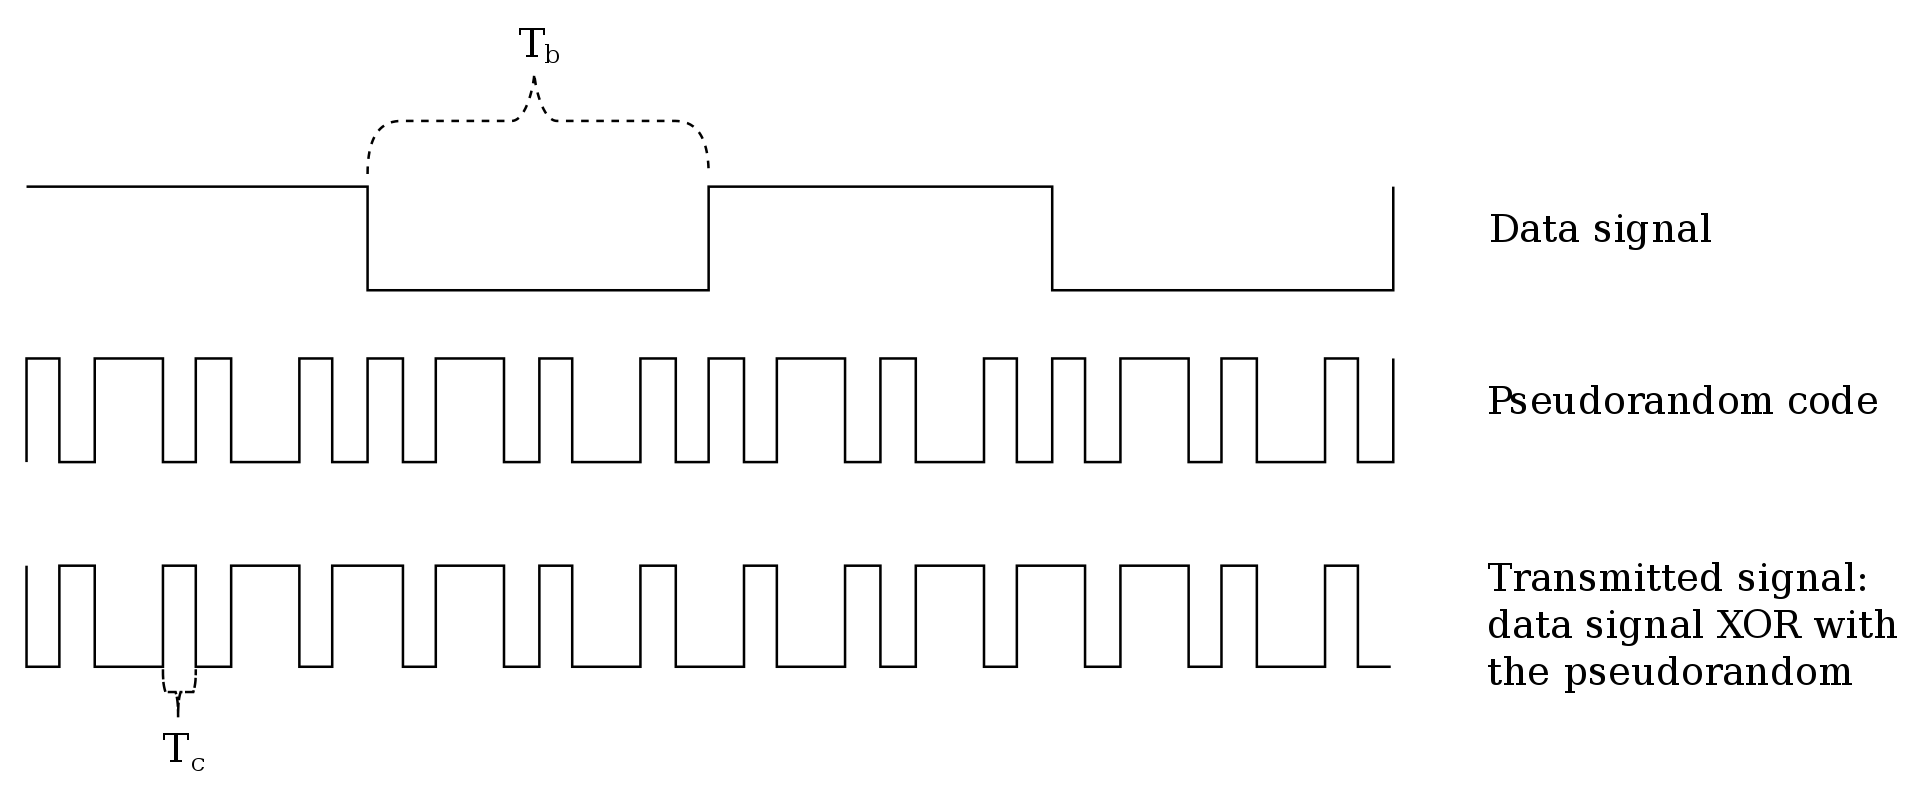
\includegraphics[scale=0.2]{img/Generation_of_CDMA.svg.png}
      \caption{Generazione del segnale CDMA trasmesso }
      \label{fig:Signals}
    \end{figure}

    Il rapporto tra i due periodi è definito come \textit{ Spreading Factor } e come requisito è stato posto a 16:
    $$ \frac{T_b}{T_c} = 16 $$

    I codici devono essere scelti in modo tale che la correlazione tra i vari segnali dei diversi utenti sia il più vicino
    possibile a zero. Nel synchronous CDMA si può sfruttare la proprietà matematica di \textit{ortogonalità} tra vettori 
    che rappresentano stringhe di dati. Due vettori $a$ e $b$ si dicono ortogonali  se vale la seguente relazione:
    $$ a \cdot b = 0 $$

    Ogni utente deve usare un codice ortogonale a quello di tutti gli altri. Nella tabella di seguito viene riportato
    un esempio di vettori $cw_1, cw_2 \in \mathbb{Z}^{16} $  ortogonali tra di loro, i bit $0, 1$ vengono rappresentati 
    rispettivamente dai simboli $-1, 1$:

    \begin{table}[H]
      \centering
      \begin{tabular}{| c | c | c | c | c | c | c | c | c | c | c | c | c | c | c | c | c | c |}\hline
        vector & \multicolumn{16}{|c|}{bit} & Prodotto Scalare \\ \hline
        \textbf{$cw_1$} &1&1&-1&1&-1&-1&-1&1&1&-1&-1&-1&1&1&-1&1& - \\ \hline
        \textbf{$cw_2$} &1&-1&1&-1&1&-1&-1&-1&1&1&-1&-1&-1&1&-1&-1& -\\ \hline
        \textbf{$cw_{1,i} * cw_{2,i}$} &1&-1&1&-1&1&-1&-1&-1&1&1&-1&-1&-1&1&-1&-1& 0 \\ \hline
      \end{tabular}
      \caption{Vettori Ortogonali}
      \label{tab:orthogonal vectors}
    \end{table}

    \subsection{Applicazioni}
     Il \textbf{CDMA} è il protocollo di accesso a canale condiviso più diffuso nelle reti wireless e nelle tecnologie
     cellulari. Deriva da una tecnologia usata per implementare il \textbf{GPS} (\textit{Global Position System}) ed è 
     stato usato in :
     \begin{itemize}
      \item \textit{Globastar network}, con il nome di CDMA2000, ed altre compagnie telefoniche
      \item \textit{UMTS 3G} come protocollo di accesso multiplo standard
      \item \textit{OmniTRACS satellite system}, per trasporti logistici.
     \end{itemize}
  \subsection{Esempio utilizzato}\label{Esempio}
    Al fine di verificare il corretto funzionamento del ricevitore, è stato seguito un caso reale di ricezione di due bit 
    in un ricevitore CDMA. Facendo riferimento ai codici ( \textit{code words} ) della tabella \ref{tab:orthogonal vectors},
    si è considerato uno scenario in cui il primo utente trasmette il simbolo $1$, mentre un secondo utente trasmette il 
    simbolo $-1$. Per le proprietà fisiche dell'interferenza, se 2 segnali interferenti sono in fase, essi si sommano e si
    crea un segnale la cui ampiezza è la somma delle ampiezze, altrimenti si sottraggono e creano un segnale con un'ampiezza pari alla differenza 
    delle ampiezze. Nel mondo digitale, questo comportamento può essere rappresentato dalla somma componente per componente
    dei vettori trasmessi.

    Nella seguente tabella \ref{tab:interference pattern}, il simbolo trasmesso è modulato con la rispettiva \textit{code word}, ottenendo un
    \textit{chip stream} per ogni utente. Ogni chip stream trasmesso interferisce con gli altri trasmessi nello stesso 
    istante, formando l'\textit{interference pattern}, cioè il segnale realemente ricevuto dai ricevitori.

    \begin{table}[H]
      \centering
      \begin{tabular}{| c | c | c | c | c | c | c | c | c | c | c | c | c | c | c | c | c |}\hline
        \texttt{data} & \multicolumn{16}{|c|}{\texttt{value}} \\ \hline
        $d_1$ & \multicolumn{16}{|c|}{$1$} \\ \hline
        $d_2$ & \multicolumn{16}{|c|}{$-1$}\\ \hline
        $cw_{1,i} * d_1$ &1&1&-1&1&-1&-1&-1&1&1&-1&-1&-1&1&1&-1&1 \\ \hline
        $cw_{2,i} * d_2$ &-1&1&-1&1&-1&1&1&1&-1&-1&1&1&1&-1&1&1 \\ \hline
        \textit{interference pattern} &0&2&-2&2&-2&0&0&2&0&-2&0&0&2&0&0&2 \\ \hline
      \end{tabular}
      \caption{Interferenza tra trasmettitori}
      \label{tab:interference pattern}
    \end{table}

    \subsubsection{Ricostruzione del segnale}\label{ricostruzione}
    Per ricostruire il segnale, un ricevitore moltiplica ogni componente dell'\textit{interference pattern} con la propria \textit{code
    word}. Il vettore $r$ ottenuto è dato in input ad un \textit{Decisore Hard A Soglia} il quale decide il bit da porre in 
    uscita. La decisione è presa nel seguente modo:

    \begin{itemize}
      \item se $\sum\limits_{i=1}^{16} r_i \geq 0 $ allora \textit{bitstream} $= 1$
      \item se $\sum\limits_{i=1}^{16} r_i < 0 $ allora \textit{bitstream} $= 0$
    \end{itemize}

    Nell'esempio considerato i ricevitori effetturanno le seguenti operazioni:

    \begin{figure}[H]
      \centering
      \begin{tabular}{| c | c | c | c | c | c | c | c | c | c | c | c | c | c | c | c | c | c | c |}\hline
        \texttt{data} & \multicolumn{16}{|c|}{\texttt{value}} & Somma & Bit deciso\\ \hline
        $r_i * cw_{1,i}$ &0&2&2&2&2&0&0&2&0&2&0&0&2&0&0&2&16&1 \\ \hline
        $r_i * cw_{2,i}$ &0&-2&-2&-2&-2&0&0&-2&0&-2&0&0&-2&0&0&-2&-16&0 \\ \hline
      \end{tabular}
      \label{tab:Decisore}
    \end{figure}

    Come si nota dalla tabella, i ricevitori sono in grado di ricostruire il bit trasmesso originariamente ( primo utente
     $1$, secondo utente $0$) come specificato in \ref{Esempio} .

\section{Architettura}
  \subsection{Diagramma a Blocchi}
    Nella Figura \ref{fig:Architettura} è rappresentato il diagramma a blocchi per il ricevitore CDMA.
      \begin{figure}[H]
      \centering
      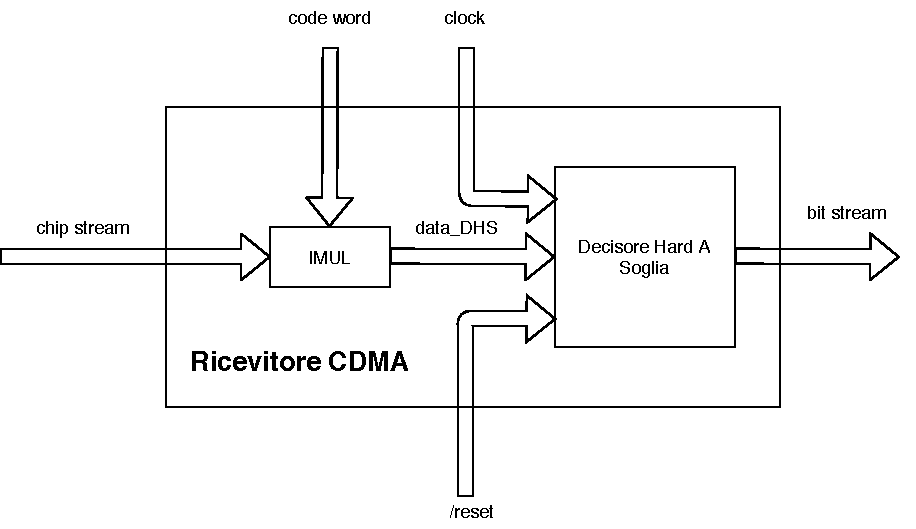
\includegraphics[scale=0.75]{img/Architettura.pdf}
      \caption{ Diagramma a blocchi dell'architettura usata }
      \label{fig:Architettura}
    \end{figure}
    In particolare vengono effettuate le operazioni descritte in \ref{ricostruzione} in modo tale da risalire al bit 
    trasmesso. Per quanto riguarda il \textit{clock} questo ha una frequenza pari al \textit{chip rate}, cioè la frequenza
    $\frac{1}{T_c}$ con cui variano i bit della \textit{code word}.
  \subsection{Implementazione}
    Per quanto riguarda l'implementazione, il Ricevitore CDMA è descritto tramite un misto tra l'architettura strutturale
    e dataflow. Infatti, questo si compone di un \textit{Decisore Hard A Soglia} il cui ingresso segue sempre il 
    prodotto tra la propria \textit{code word} e il \textit{chip stream} ricevuto o \textit{interference pattern} secondo
    quanto detto in \ref{tab:interference pattern}.
    Questi ultimi sono stati rappresentati tramite degli interi che di 
    default sono su 32bit, ma per rendere più efficiente il sistema, è stato specificato il range di valori, in modo tale
    che il sintetizzatore faccia le dovute ottimizzazioni. 
    \begin{figure}[H]
      \centering
      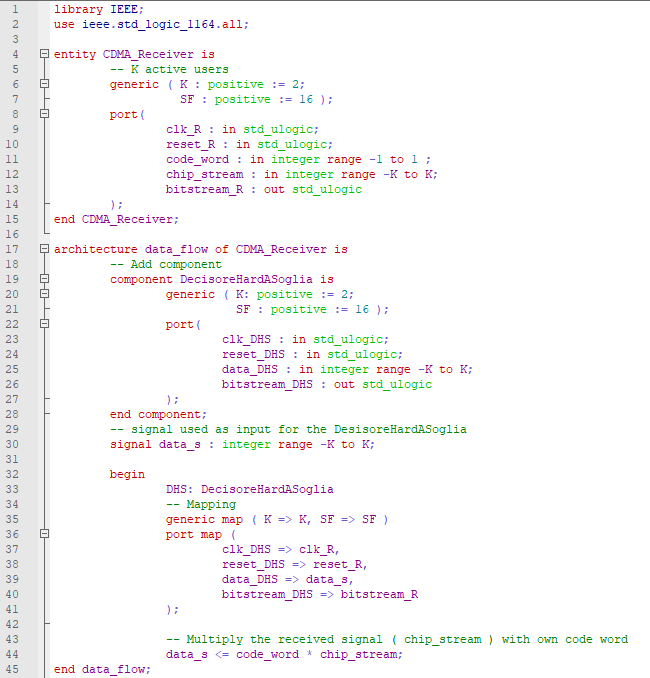
\includegraphics[width=\textwidth]{img/CDMAReceiver.png}
      \caption{Descrizione VHDL CDMA Receiver}
      \label{fig:vhdl:cdma}
    \end{figure}

    Il \textit{Decisore Hard A Soglia} è stato descritto tramite l'architettura di tipo Behavioral in modo tale da 
    specificare cosa accade quando arriva il fronte di salita del clock. Superata la fase iniziale di reset, il Decisore
    effettua la somma dei dati ricevuti ingresso ad ogni ciclo di clock, tenendo nel segnale \textit{waitData} quanti dati
    ha già contato. Un volta sommati \textit{SF} dati si può procedere con la decisione seguendo quanto descritto in 
    \ref{ricostruzione}.
    \begin{figure}[H]
      \centering
      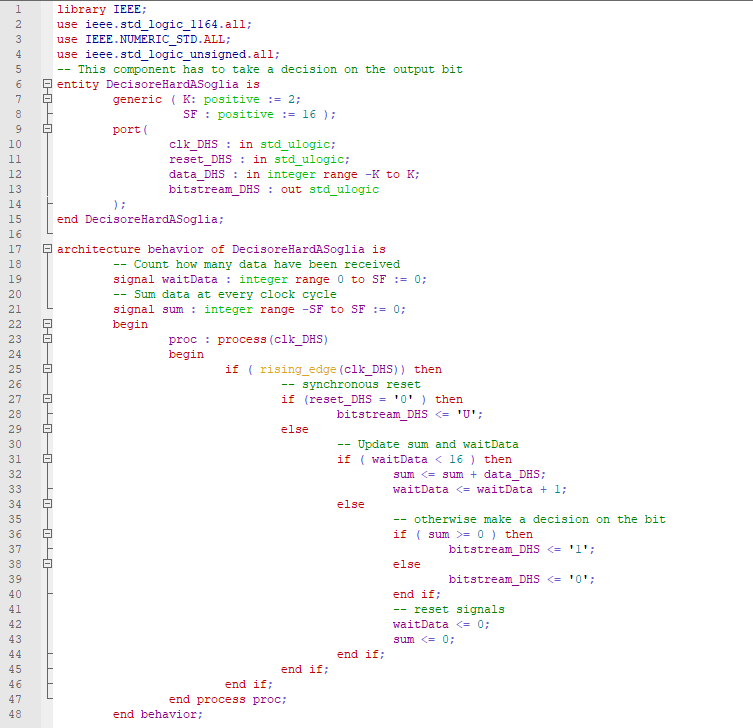
\includegraphics[width=\textwidth]{img/DecisoreHardASoglia.png}
      \caption{Descrizione VHDL Decisore Hard A Soglia}
      \label{fig:vhdl:DHS}
    \end{figure}  

  \subsection{Test-plan}
    Per testare il ricevitore sono stati creati 2 testbench che seguono l'esempio descritto in \ref{Esempio}. In particolare,
    è stato ricreato lo scenario in cui 2 utenti trasmettono nello stesso istante rispettivamente il bit $1$ e il bit $0$ 
    mentre 2 ricevitori con le stesse code word dei trasmettitori stanno in ascolto.
    I test devono verificare che i ricevitori riescano a ricevere i bit giusti nonostante l'intereferenza. Quindi:
    \begin{itemize}
      \item Ricevitore 1 deve decidere il bit $1$
      \item Ricevitore 2 deve decidere il bit $0$
    \end{itemize}
    \subsubsection{Testbench 1}
    Entrambi i test sono stati effettuati con un periodo di clock pari a 10 ns, quindi una frequenza di \SI{100}{\mega\hertz}.
    \begin{figure}[H]
      \centering
      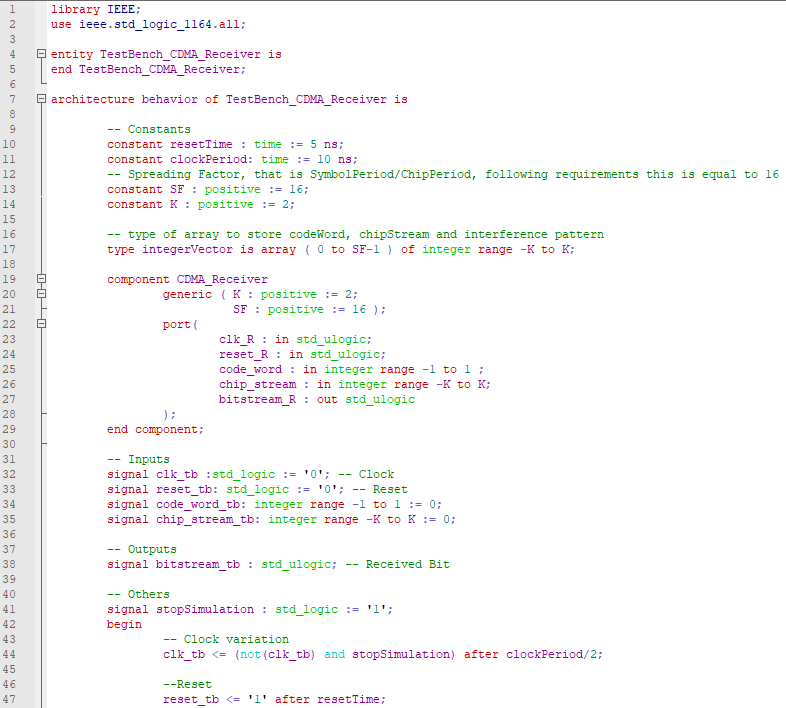
\includegraphics[scale=0.9]{img/TB1.png}
      \label{fig:vhdl:tb1}
    \end{figure}
    \begin{figure}[H]
      \centering
      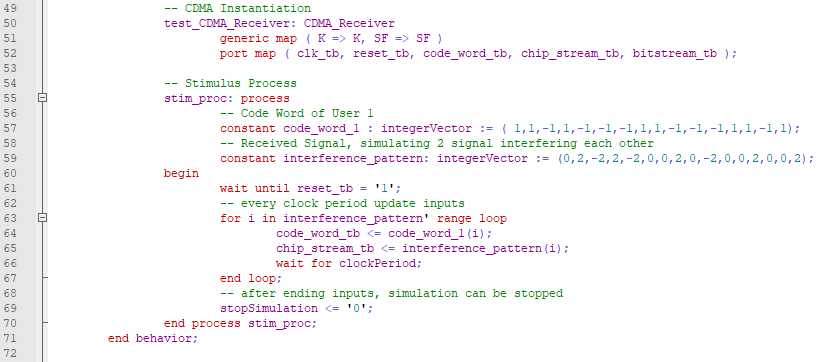
\includegraphics[width=\textwidth]{img/TB1.1.png}
      \caption{Testbench 1: il trasmettitore invia il bit '1'}
      \label{fig:vhdl:tb11}
    \end{figure}

    \begin{figure}[H]
      \centering
      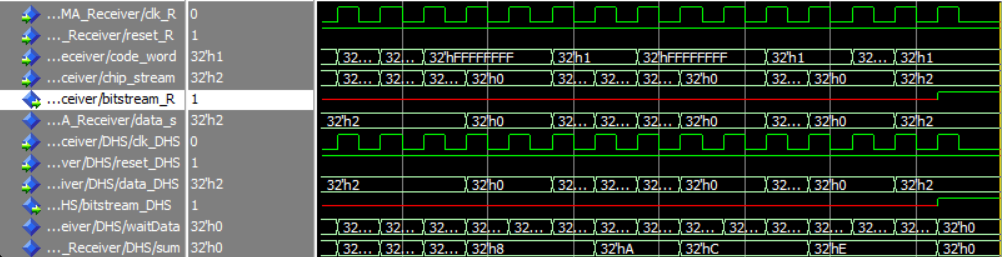
\includegraphics[width=\textwidth]{img/Wave1.png}
      \caption{Simulazione ricezione 1}
      \label{fig:vhdl:wave1}
    \end{figure}
    Come si può vedere in \ref{fig:vhdl:wave1}, l'uscita \textit{bitstream} del ricevitore viene settata ad 1 una volta 
    che tutto il chip stream è stato ricevuto.

    \subsubsection{Testbench 2}
    Di seguito è riportata solo la parte relativo allo Stimulus process del secondo test dato che il resto è uguale al primo.
    \begin{figure}[H]
      \centering
      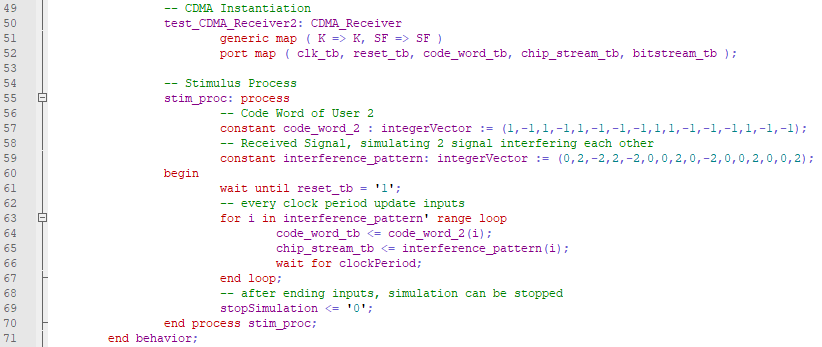
\includegraphics[scale=0.7]{img/TB2.png}
      \caption{Testbench 2: il trasmettitore invia il bit '0'}
      \label{fig:vhdl:tb2}
    \end{figure}

    \begin{figure}[H]
      \centering
      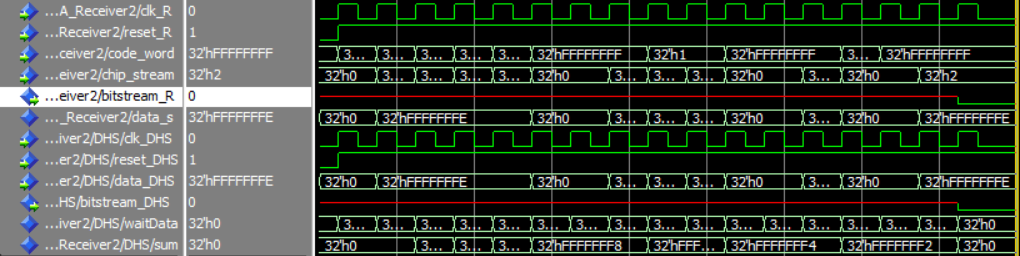
\includegraphics[width=\textwidth]{img/Wave2.png}
      \caption{Simulazione ricezione 0}
      \label{fig:vhdl:wave2}
    \end{figure}
    Il test conferma che il ricevitore 2 riesce decidere il bit 0 a partire dallo stesso chip stream ricevuto dal primo 
    ricevitore. 

\section{Sintesi} 
  La sintesi è stata effettuta tramite il tool Vivado applicando come unico constraint:
  \begin{itemize}
    \item{Clock: 10ns}
  \end{itemize}
  \subsection{Utilizzo}
    \begin{figure}[H]
      \centering
      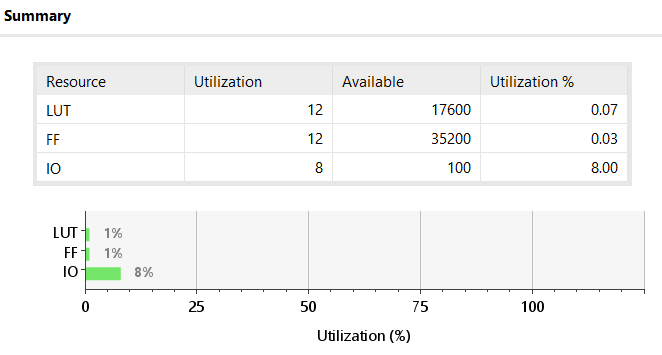
\includegraphics[width=\textwidth]{img/Utilizzo.png}
      \caption{Percentuale di utilizzo}
      \label{fig:utilizzo}
    \end{figure}
    Le risorse utilizzate sono poche rispetto a quelle disponibili. Il maggior utilizzo si ha sull'I/O in quanto vengono 
    utilizzati 8 pin su 100 disponibili ( 3 chipstream, 2 code word, 1 clock, 1 /reset, 1 bitstream ).
  \subsection{Massima frequenza di utilizzo}
    \begin{figure}[H]
      \centering
      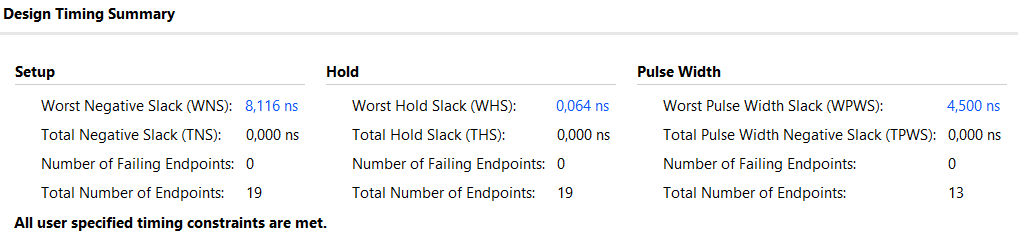
\includegraphics[width=\textwidth]{img/FrequenzaMassima.png}
      \caption{Timing}
      \label{fig:timing}
    \end{figure}
    Il ricevitore così descritto è in grado di rispettare il vincolo sul clock imposto ottenendo un \textbf{WNS} di \SI{8.116}{\nano\second},
    quindi è possibile tollerare una frequenza massima pari a:
    $$ f_{max} = \frac{1}{T'_{clock}} = \frac{1}{T_{clock}-T_{slack}} =  \text{\SI{530.78}{\mega\hertz}} $$  
  \subsection{Cammino Critico}
    Il cammino critico che produce il $T_{slack}$ mostrato in \ref{fig:timing} è il seguente:
    \begin{figure}[H]
      \centering
      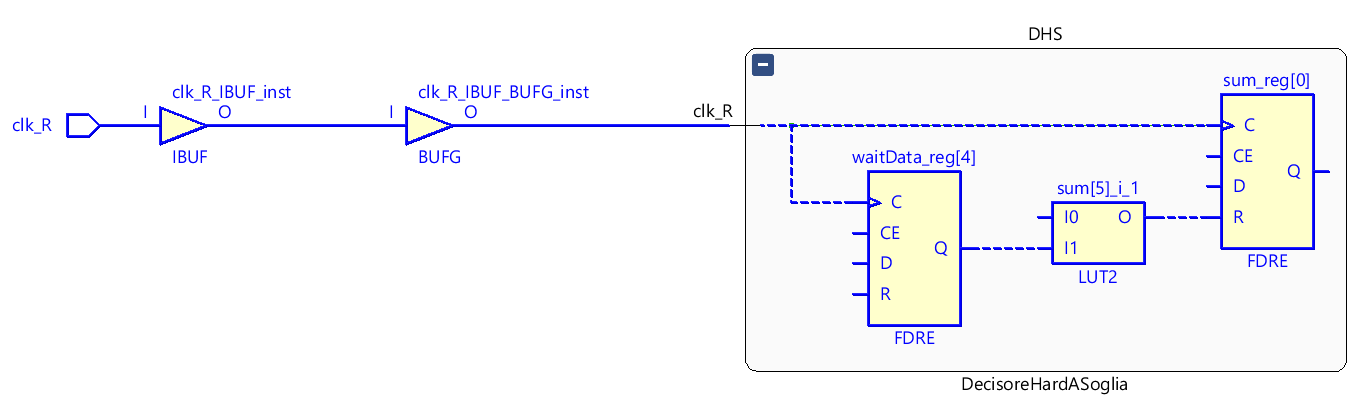
\includegraphics[width=\textwidth]{img/CamminoCritico.png}
      \caption{Cammino Critico}
      \label{fig:critico}
    \end{figure}
  \subsection{Consumo di Potenza}
    Dal consumo di potenza si può notare quanto l'algoritmo implementato ha necessità computazionali basse, dato che la 
    maggior parte della potenza è richiesta a mantenere attivo il dispositivo più che ad effettuare le dovute operazioni.
    \begin{figure}[H]
      \centering
      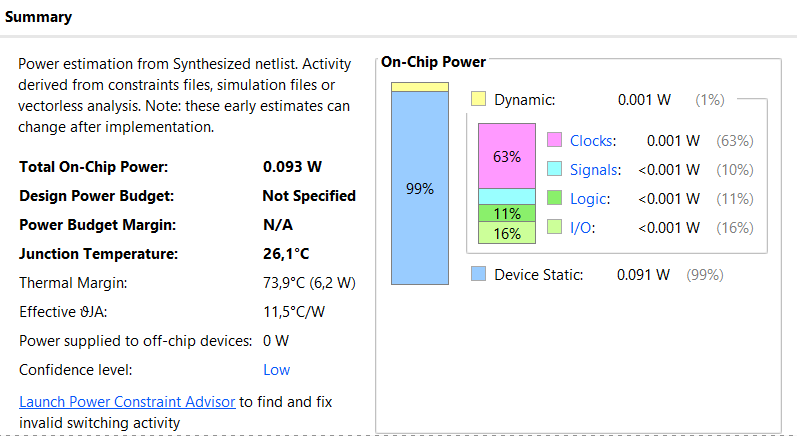
\includegraphics[width=\textwidth]{img/Power.png}
      \caption{Percentuale Consumo di Potenza}
      \label{fig:power}
    \end{figure}
\section{Conclusioni}
  In questo progetto è stato descritto, implementato e sintetizzato un Ricevitore CDMA che riceve un segnale, somma
  dei segnali trasmessi in quell'istante, ma è in grado comunque di ricostruire il segnale trasmesso dal suo interlocutore
  nonostante le interferenze. I test hanno verificato il corretto funzionamento dei ricevitori, andando a valutare il 
  comportamento in uno scenario realistico. Inoltre, la sintesi ha mostrato che il dispositivo è in grado di sopportare 
  frequenze fino a \SI{530.78}{\mega\hertz} quindi a tale frequenza e considerando uno \textit{Spreading Factor} pari a 16,
  l'intera sequenza di \textit{chip stream} è ricevuta in $T'_{clock}*16 = \text{\SI{30.11}{\nano\second}}$. 
\end{document}
